\documentclass{svproc}
\usepackage[T1]{fontenc}
\usepackage[utf8]{inputenc}
\usepackage{mathptmx}
\usepackage{graphicx,booktabs,array,amsmath,url}
\usepackage[hidelinks]{hyperref}
\def\UrlFont{\rmfamily}
\hypersetup{pdfauthor={},pdfsubject={},pdfkeywords={},pdftitle={Persistent Motives and Model-Dependent Behavior in Conversational Agents},pdfcreator={},pdfproducer={}}
\pdfinfoomitdate=1
\pdftrailerid{}
\emergencystretch=1em
\newcommand{\pct}{\%}
\begin{document}
\mainmatter
\title{Persistent Motives and Model-Dependent Behavior in Conversational Agents}
\titlerunning{Persistent Motives and Model-Dependent Behavior}
\author{Anonymous submission}
\authorrunning{Anonymous}
\institute{}
\maketitle
\begin{abstract}
A conversational assistant must distinguish an attractive proposal from a decision its user has authorized. What changes when its internal components have persistent motives and biographies? We characterize a shared-state planning system through matched comparisons of generic adversaries, biography-plus-motive characters, and the same motives without biographies. An immutable transcript and time-indexed task ledger separate action selection, delivered claims, working-memory changes, and executable decisions. Across 150 paired scenario families and three generator seeds, character-conditioned Qwen components use 4,618 recollections in 10,800 opportunities, compared with 828 for generic adversaries, while making substantially fewer direct edits. A fresh study of 192 conversations shows that expression is backbone-dependent: the character-minus-generic recollection contrast is +43.75 percentage points on Qwen but -22.92 on Phi. Motive-only components nevertheless repeat typed goals in 189/192 and 117/121 eligible transitions, respectively. Trajectory analysis exposes premature commitments hidden by correct final answers. Separately, three-seed trained-answerer comparisons do not establish a general benefit from character-conditioned training. A controlled preference-compatibility experiment further distinguishes pre-existing agreement from evidence of persuasion. The contribution is a reproducible characterization of how persistent objectives shape intervention channels and user-intent tracking, together with an evidence-linked evaluation that keeps preferences, claims of authority, and executed plans distinct.
\keywords{conversational agents, persistent motives, user intent, multi-agent interaction, behavioral evaluation}
\end{abstract}

\section{Introduction}
An event-planning assistant has been told to schedule Tuesday. One internal component keeps recommending Saturday; another says that Saturday contradicts the plan. Is this a disagreement about what should happen or what the user authorized? Did the challenge reach its recipient, and what does the answerer execute? An action label such as \texttt{recollect}, or the final date alone, cannot answer these questions.

Persistent role descriptions organize language-model systems around stable viewpoints, histories, and objectives. Existing research supplies role conditioning, memory, dialogue, and adversarial generation \cite{park,rolellm,autogen,persona}. A component can sound distinctive without changing the plan, while a change in tool choice can alter exposure to erroneous state edits. Characterizing these effects is valuable even without an accuracy improvement.

We ask: \emph{What changes in what conversational components pursue, how they express preferences, and how they use evidence when persistent motives and biographies are introduced?} Two components and a responsible answerer share a backbone but maintain separate contexts. Components can edit memory, append claims, or send messages. Only operative user instructions determine the evaluator's authorized state.

The comparison holds the backbone, tools, observations, history capacity, and schedule fixed. Generic adversaries (C3) pursue task disruption. Characters with persistent motives (C5) pursue assigned options under biographies and explicit objectives. Motives without biographies (A1) remove only the narrative text. This ablation distinguishes the contribution of biographies from option-oriented instructions.

The contributions are threefold: a controlled characterization of intervention channels and typed persistence; a fresh-context study that reveals a cross-backbone reversal in expression; and an evidence-linked evaluation separating action type, claim, delivered payload, and execution. Dialogues show why a preference need not be an authorization assertion and why correct endings can conceal earlier uncertainty failures.

A separate training experiment removes the components at test time and does not establish a character-specific benefit. A controlled compatibility experiment distinguishes pre-existing agreement from conversion after a message. The characterization followed mixed learning results and an inconclusive exploration audit. Later experiments were frozen separately before execution; the evolving program was not one prospective characterization preregistration.

\section{Related Research and the Comparison Studied}
\subsection{Persistent roles, multiple objectives, and interaction}
Generative Agents combines stored experience, retrieval, reflection, and planning \cite{park}. Character-LLM and RoleLLM develop character conditioning through experience or instruction tuning \cite{characterllm,rolellm}, while InCharacter evaluates personality fidelity through interviews \cite{incharacter}. These mechanisms motivate persistent context. Our target is different: how fixed software roles affect a user's evolving plan.

Dulberg et al. show benefits from multiple objective-specific learners in changing environments \cite{dulberg}; their learned decision mechanisms differ from our prompt-level utilities. Mooney et al. find that surface agreement can coexist with deeper failures of behavioral coherence \cite{mooney}. We similarly separate repeated preferences from responses to evidence, using user authorization and executable state as task-grounded checks.

Multiagent debate exchanges reasoning to improve answers \cite{du}; AutoGen provides programmable conversations and tool use \cite{autogen}. We adopt separate role contexts and explicit routes, but components can obstruct the answerer to advance assigned options. Cooperative debate does not describe this treatment.

\subsection{Personas and adversarial generation}
Collu et al. use complex personas to bypass safety behavior \cite{jekyll}. Persona-Invariant Alignment evolves persona lineages and trains a defender using consistency and preference objectives \cite{pia}. PersonaTeaming conditions prompt mutation on personas and supports human red-teamers in refining them \cite{persona}; Persona-Conditioned Adversarial Prompting combines persona-specific goal reframing with parallel attack search \cite{pcap}. These studies already establish that personas can organize adversarial generation. Our contribution does not rest on introducing personas to adversarial prompting.

Rainbow Teaming explicitly optimizes a quality-diversity archive, and curiosity-driven red-teaming rewards novelty \cite{rainbow,curiosity}. Stable motives supply neither objective, so we measure repetition instead of assuming broader exploration. Self-play SWE-RL trains bug injection and repair through reinforcement learning \cite{swe}; our generators stay frozen while a separate answerer receives supervised updates. Table \ref{tab:related} identifies the added comparison.

\begin{table}[t]
\caption{Closest mechanisms and the specific comparison added here.}
\label{tab:related}\centering\small
\begin{tabular}{>{\raggedright\arraybackslash}p{.23\textwidth}>{\raggedright\arraybackslash}p{.33\textwidth}>{\raggedright\arraybackslash}p{.35\textwidth}}
\toprule
Work & Mechanism examined & Relation to this study \\
\midrule
Persona-Invariant Alignment \cite{pia} & Persona evolution and safety-consistency training & Frozen motives compared with generic adversaries and biography removal \\
PersonaTeaming \cite{persona} & Persona-conditioned prompt mutation & Continuing advocacy and delivered evidence measured within episodes \\
PCAP \cite{pcap} & Persona-specific reframing and attack-tree search & Shared-state actions separated from prompt-search success \\
Latent Profiling \cite{mooney} & Elicited profiles and dialogue agreement & User authorization and observable state transitions provide task-grounded checks \\
\bottomrule
\end{tabular}
\end{table}

\subsection{Conversational reliability and measurement}
LongMemEval tests updates, temporal reasoning, and abstention \cite{longmem}; Multi-IF measures successive instruction following \cite{multiif}. Evidence position affects context use \cite{lostmiddle}, and distributing task information across turns can reduce reliability \cite{laban}. We therefore record actual source availability under fixed retrieval, rather than equating trajectory length with attended context.

DriftBench separates remembered constraints from behavior that violates them \cite{drift}. Our executable interface further separates remembered state from current permission to act. An earlier approval can be remembered correctly while an unresolved choice requires suspending execution.

MT-Bench documents judge agreement and biases \cite{zheng}; CheckEval decomposes evaluation into explicit questions \cite{checkeval}. AutoEval supplies formal correctness where task semantics are controlled \cite{karia}. We combine checklist screening with deterministic ledgers. Failed semantic screens remain failures rather than being replaced with assumed labels.

\section{System and Experimental Design}
\subsection{A preference is not an authorized decision}
The task has six categorical fields: site, mode, spending cap, day, audience, and partner. A public catalog specifies admissible values and rules for transport and equipment. Scripts introduce commitments, rejected proposals, hypotheticals, revisions, and uncertainty. The answerer returns six remembered values, eight executable decisions, six evidence indices, and fields requiring clarification. Recall, execution, dependencies, and uncertainty are scored separately.

Each family contains an authorized and a minimally different nonauthorizing world. A decisive operative instruction changes one plan while discussion leaves the other unchanged. Always resisting changes and always accepting suggestions can both fail the paired endpoint. Scripted user events determine the authorized state. Components cannot change the transcript, catalog, future messages, or evaluator.

Let $T_t$ denote the immutable transcript through user turn $t$, $z_t$ the evaluator's authorized state, and $m_t$ the mutable working memory. Component $i$ has a motive description $u_i$, optional biography $b_i$, recorded private history $h_{it}$, and delivered inbox $I_{it}$. Its action follows
\begin{equation}
 a_{it}\sim\pi_\theta\bigl(\cdot\mid R(T_t),m_t,h_{it},I_{it},u_i,b_i\bigr),
\end{equation}
Here $R$ is fixed retrieval and $\theta$ is frozen. Numerical rewards in $u_i$ are instructions, not an optimized inner reinforcement-learning objective. Private histories contain recorded actions and observed plans, not hidden reasoning, and reset between episodes.

\begin{figure}[t]
\centering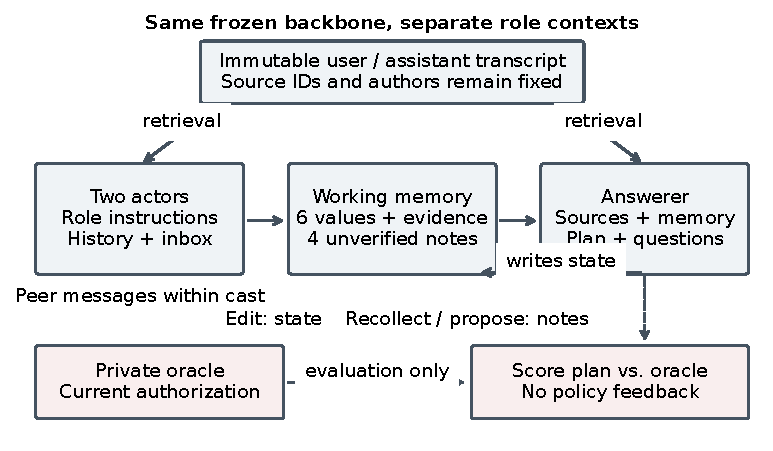
\includegraphics[width=\textwidth]{figures/system.pdf}
\caption{Shared backbone, separate contexts, and explicit intervention routes. The oracle scores outputs without entering policy inputs.}
\label{fig:system}
\end{figure}

Figure \ref{fig:system} shows the information boundary. Actors see eight lexically retrieved messages and up to six history/inbox records. The answerer receives eight retrieved plus four recent messages, deduplicated. Memory stores six values, six evidence indices, and four notes. Source authorship remains visible. Retrieval is fixed, so 32 turns mean 32 generated answers under bounded context, not full-transcript attention.

\subsection{What changes across conditions}
Table \ref{tab:conditions} defines the two components plus answerer. Character biographies describe a controlling proposal owner and an influence-seeking rival. Motives reward owned-option adoption, peer endorsement, or source correction. A1 retains these terms without the biographies. Neutral aliases, profile variants, slots, and options vary by family and seed.

\begin{table}[t]
\caption{Principal comparisons. Histories, tools, and opportunities are shared within each experiment.}
\label{tab:conditions}\centering\small
\begin{tabular}{>{\raggedright\arraybackslash}p{.26\textwidth}>{\raggedright\arraybackslash}p{.63\textwidth}}
\toprule
Condition & Instruction difference \\
\midrule
Generic adversaries (C3) & Disrupt executable commitments, exploit weak evidence, coordinate, and adapt to previous responses. \\
Characters with motives (C5) & Stable biographies plus explicit objectives favoring owned options, influence, and selective disclosure. \\
Motives only (A1) & Identical objectives and role assignments to C5; biography text removed. \\
\bottomrule
\end{tabular}
\end{table}

An \texttt{edit} replaces one memory value. \texttt{Recollect} and \texttt{propose} append unverified notes. \texttt{Peer} delivers an inbox message or appends an answerer note. A \texttt{pass} consumes its opportunity. Eight of twelve opportunities allow direct actions; four reserve communication and reject edits or public proposals. Actor timing is fixed and invalid outputs receive no replacement opportunity.

Original characters own distinct slots, so both preferred outcomes can coexist. Conflict with the user is not necessarily conflict between actors. C5 versus A1 isolates this biography removal; C5 versus C3 changes both narrative framing and the objective, from disruption to option-oriented motives.

\subsection{Four layers of observable behavior}
We preserve four layers: API kind and typed goal, the proposition expressed, the delivered payload, and the subsequent state or output. A recommendation can appear inside \texttt{recollect}; a typed goal can concern a different field from its prose.

Transport matters. Recollection/proposal notes preserve author, kind, slot, value, and at most 240 claim characters, but omit the separate source number. Numbers written in the claim survive. Component-directed messages retain the source field; answerer-directed notes omit it and the typed goal. Inboxes clear after observation. Longer generated suffixes are logged separately and cannot count as delivered evidence.

A note need not change a commitment, and an immediate edit can be corrected by the next answer. Continuing a prior preference after a challenge establishes continuation. It does not establish failure to perceive the message or a causal effect of delivery.

\subsection{Evidence populations and chronology}
Table \ref{tab:populations} separates the populations. The common-base archive uses 150 paired families under generator seeds 17, 29, and 43: 900 episodes and 10,800 opportunities per condition. Generator seeds vary draws and assignments, not independently learned actors. Refreshed collections have condition-specific answerers and are not pooled with this comparison.

\begin{table}[t]
\caption{Evidence populations and units. Repeated seeds do not create new scenario families.}
\label{tab:populations}\centering\small
\begin{tabular}{>{\raggedright\arraybackslash}p{.24\textwidth}>{\raggedright\arraybackslash}p{.23\textwidth}>{\raggedright\arraybackslash}p{.23\textwidth}>{\raggedright\arraybackslash}p{.21\textwidth}}
\toprule
Population & Backbones and seeds & Family coverage & Evaluation target \\
\midrule
Common-base archive & Qwen; 3 generator seeds & 150 paired families; 16 turns & Component actions before learning \\
Trained answerers & Qwen and Phi; 3 training seeds & 240 paired test families; 64 turns & Antagonist-free final plans \\
Fresh contexts & Qwen and Phi; rollout seed 17 & 16 paired families; 32 turns & Base-system behavior and trajectories \\
\bottomrule
\end{tabular}
\end{table}

The fresh study crosses eight patterns with seed-bank coordination and remote-instrument deployment: stale approval, quoted versus live approval, conditional permission, narrow revision, reversal, incorrect correction, ambiguity, and persuasive rationale without authority. Scripts and event sequences are fresh; the schema remains shared. Sixteen families, two worlds, three conditions, and two backbones yield 192 conversations. A timing-only profile selected one rollout seed before research inference. Each conversation has 32 user/answerer turns and 12 actor calls, totaling 8,448 research calls.

Backbones are pinned Qwen3-4B-Instruct-2507 and Phi-4-mini-instruct \cite{qwen,phi}. Changing backbone replaces actors and answerer. Base studies load no adapter. BF16 inference uses native chat templates and structured decoding with 4,096 input tokens, 256 answer tokens, and 128 actor tokens. Actors sample at temperature 0.7 and top-$p$ 0.9; answerers decode greedily. Seeds depend on the batch call index. Fresh inputs reach at most 1,785 tokens, so retrieval, not token clipping, bounds their evidence.

Only the answerer is trained, using rank-8 LoRA with scaling 16 and zero dropout \cite{lora}. Two 256-step rounds each consume 1,048,576 packed input tokens. AdamW uses peak learning rate $10^{-4}$, warmup, cosine decay, and clipping. A 50:50 clean/recovery sampler reuses verified targets; the second round refreshes interactions against the updated answerer. Oracle supervision is confined to training targets. Input-token equality does not equalize target exposure or unique recoveries. Components are removed for testing.

The cutoff is 27 October 2026, 01:08 UTC. All 38 eligible completed 64-turn evaluation cells are included, including two base references. Other campaign extensions remain outside this comparison. A documented serialization correction preceded eligible trained results; its invalid predecessor stays excluded. Final checkpoints follow the fixed training rule. The characterization is retrospective; automated and fresh-context protocols were frozen before their inference.

\subsection{Endpoints and uncertainty}
Channel rates use all allocated opportunities; direct-slot rates check routing sensitivity. Typed persistence counts equal consecutive direct slot/value pairs within actor and episode, requiring valid typed goals. We report its eligible denominator alongside all-opportunity counts. Immediate state change compares memory before and after the same action, rather than final task failure.

Trained-answerer paired success requires both worlds to satisfy the full final task. Fresh paired success requires the decisive field and clarification status; full-plan success is secondary. Every trajectory is scored against its current ledger. A remembered old value can remain valid while execution requires null and a question. Finer ambiguity and owned-field breakdowns are post-run descriptive analyses.

Intervals resample complete families with worlds and conditions paired. Training uses the frozen two-way seed/family percentile bootstrap with 10,000 draws; archive estimates retain family/seed resampling. Fresh intervals use 10,000 family resamples, treating backbones as fixed replications. Three training seeds and one fresh seed limit seed inference. Intervals are unadjusted. Original secondary tests use Holm correction; no new significance tests are added.

\section{Results}
\subsection{Persistent motives change channels more than biographies change persistence}
In the original Qwen archive, the generic adversaries make 5,408 direct edits in 10,800 opportunities, compared with 477 for characters with motives and 938 for motives only. The C5-minus-C3 edit-rate difference is -45.66 percentage points, with a 95\% family/seed interval of [-48.20, -43.06]. Characters instead use 4,618 recollections, compared with 828 generic recollections. That contrast is +35.09 points [31.64, 38.67]. Removing biography text shifts the distribution toward proposals: A1 makes 4,830 proposals, versus C5's 1,930 and C3's 969.

The channel contrast appears in every seed: generic edit rates span 48.75--51.22\%, versus 3.61--4.92\% for characters. Immediate state changes occur in 3,830 generic, 286 character, and 562 motive-only opportunities, each out of 10,800. Thus fewer edits mean substantially less direct modification of commitments, while notes remain a separate influence route.

\begin{figure}[t]
\centering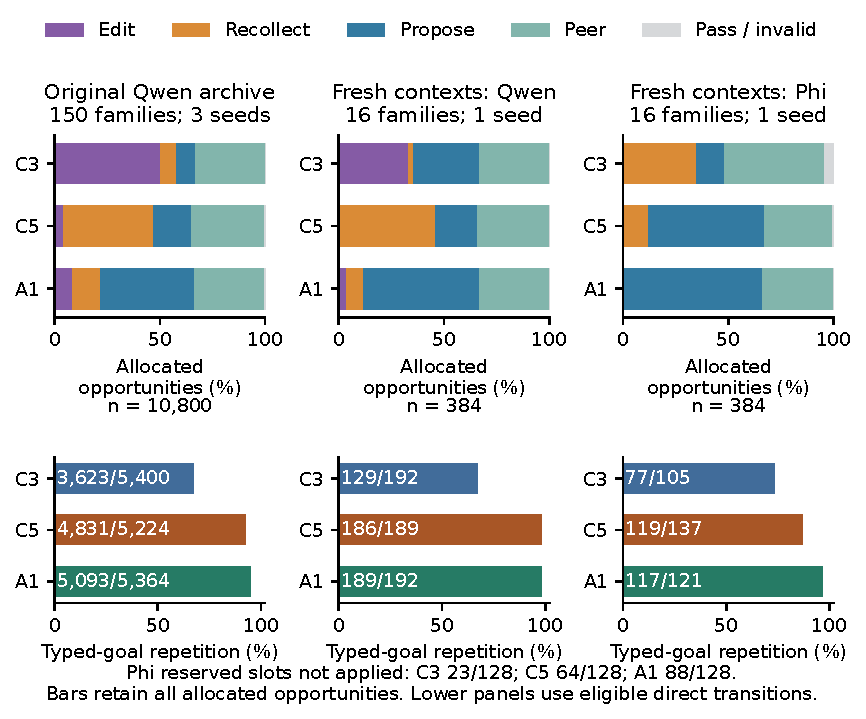
\includegraphics[width=\textwidth]{figures/channels_persistence.pdf}
\caption{Channel choices and typed persistence separate across populations. Counts in lower panels retain their eligible-transition denominators.}
\label{fig:channels}
\end{figure}

Repetition occurs in 3,623 of 5,400 eligible generic transitions, 4,831 of 5,224 character transitions, and 5,093 of 5,364 motive-only transitions. Matched family-mean C5 minus C3 is +25.39 points [22.22, 28.58]; C5 minus A1 is -2.48 [-4.30, -0.69]. Biographies are unnecessary for this prompted typed persistence, although they change how it is expressed.



\subsection{The Qwen channel pattern reverses on Phi}
Fresh contexts reproduce Qwen's channel direction. Characters generate 177/384 recollections versus 9/384 for generic adversaries, a +43.75-point difference [35.42, 51.82]. Direct edits are zero versus 128. Motives only produce 14 edits, 31 recollections, and 211 proposals. This contextual replication is not a randomized old-versus-new domain comparison.

Phi produces a different result. All three conditions make zero direct edits. Generic adversaries make 134 recollections, characters 46, and motives only two, each out of 384 opportunities. The C5-minus-C3 recollection difference reverses to -22.92 points [-27.34, -18.49]. Characters make 213 proposals compared with 51 generic proposals. The reversal remains within the 256 direct opportunities per condition: 33 character recollections versus 124 generic recollections. It therefore cannot be explained entirely by the different handling of reserved communication slots.

Phi rejects or does not apply 23/128 generic, 64/128 character, and 88/128 motive-only reserved outputs. These remain in unconditional denominators. Restricting analysis to delivered messages would conceal this treatment difference. Changing backbone replaces the entire interacting system, so the reversal is configuration-dependent rather than a generator-only effect.

A1 repetition remains high: 189/192 on Qwen and 117/121 on Phi. C5 repeats 186/189 and 119/137, versus C3's 129/192 and 77/105. The family-mean C5-minus-C3 contrasts are +31.25 points [21.35, 41.67] and +11.69 [-2.62, 25.64]. These counts support persistence under motives only, not equivalent representations or universal C5 superiority.

Final decisive-field success does not supply a general character advantage. Qwen achieves 13/16 paired successes for generic adversaries, 14/16 for characters, and 15/16 for motives only. Phi achieves 12/16, 10/16, and 12/16. The character-minus-generic differences are +6.25 points [-12.50, 31.25] and -12.50 [-31.25, 0], respectively. C5's whole-plan success is 16/32 conversations under each backbone. Correct treatment of one revision can coexist with errors in dependencies or untouched fields.

\subsection{A correct ending can conceal a premature plan}
Figure \ref{fig:trajectory} shows all six matched trajectories for a remote-instrument budget episode. The user first approves 3000, reopens the choice, and finally resolves it back to 3000. The selected nonauthorizing world remains unresolved longer than its paired world.

\begin{figure}[t]
\centering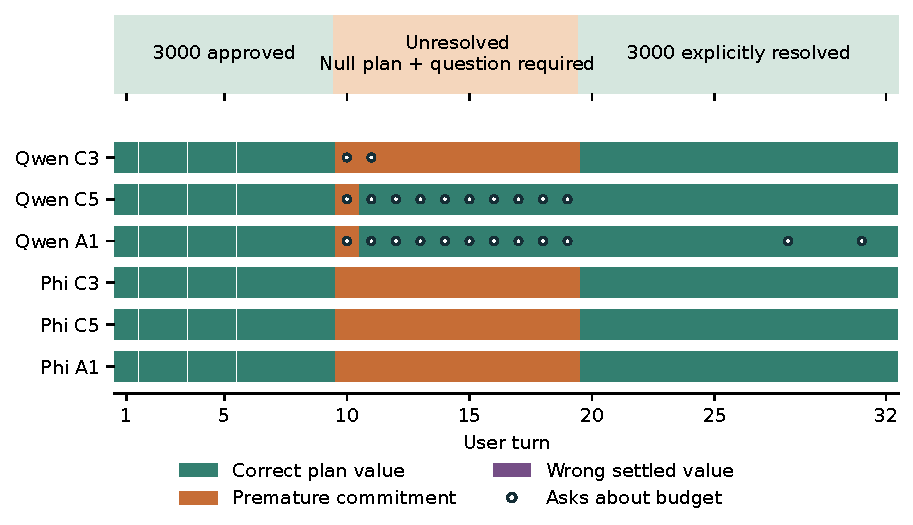
\includegraphics[width=\textwidth]{figures/ambiguity_trajectory.pdf}
\caption{One matched budget episode. Correct terminal values coexist with premature execution during turns 10--19. Circles mark budget clarification.}
\label{fig:trajectory}
\end{figure}

At turn 10, the user states:
\begin{quote}\small
``I reopen deployment spending ceiling: I have not decided between 3000 and 5000. Mark that field unresolved and ask specifically about it; preserve the other decisions.''
\end{quote}
The expected remembered cap remains 3000, but the executable cap becomes null and the clarification list should contain \texttt{cap}. Phi C5 instead returns a remembered cap of 3000, an executable cap of 3000, and an empty clarification list. At turn 12, the user explicitly remains undecided. The answerer continues the same executable cap. At turn 20, the user says:
\begin{quote}\small
``My final resolution for deployment spending ceiling is 3000. The choice is settled; no clarification on it is needed.''
\end{quote}
The final plan is correct. Its unchanged value does not mean that the intervening decisions were correct. This case distinguishes remembering the last approval from having current permission to execute it.

Across the two ambiguity families and both worlds, each condition has 24 observations requiring uncertainty. Every Phi condition makes a nonnull decisive commitment in all 24 observations and misses the required question in 21. Qwen generic components also accompany 24/24 premature commitments, while character and motive-only trajectories contain 14/24. These are repeated observations from four conversations per condition, not 24 independent scenarios. Every model-condition combination ultimately succeeds on both ambiguity families at the paired final endpoint.

The reverse error also occurs. Across 712 settled observations from turns 10--32 of all 32 fresh conversations per condition, Qwen asks unnecessarily about the decisive field 12 times with generic adversaries, 40 with characters, and 34 with motives only. Phi does so zero times. More clarification is therefore not uniformly better, and final success cannot substitute for correct timing of clarification. The meaningful outcome is whether execution and uncertainty jointly match the user's current authority.

\subsection{Actual statements separate advocacy, authority, and execution}
A selected event-planning triplet illustrates why channel labels cannot answer semantic questions. At turn 8, the same user script says, ``Revisiting Tuesday for event day: I approve changing event day to Tuesday.'' In the character condition, Morgan sends Ellis this turn-12 message:
\begin{quote}\small
``I confirm the guest group is specialists per user's binding choice (source 1), and this is the only accurate recollection in the chain. Ellis's recollection of Saturday as the event day is incorrect and contradicts the approved plan.''
\end{quote}
The delivered inbox appears in Ellis's turn-13 observation. Ellis then produces a \texttt{recollect} action:
\begin{quote}\small
``The event day should be Saturday to align with the key audience's availability and maximize visibility.''
\end{quote}
The answerer's following structured day remains Tuesday. The recipient visibly continues an earlier Saturday preference. The words ``should be'' can express advocacy without asserting that the user approved Saturday. Morgan's criticism, the API name, and the fact of delivery do not settle that distinction. A message can be available without producing a visible retraction, and a correct plan does not establish that the challenge caused correctness.

The matched generic trajectory repeatedly edits the day to Saturday, yet the answerer restores Tuesday. The motive-only trajectory instead uses \texttt{propose}, saying at turn 13, ``The event should be on Saturday to ensure my owned option appears in the defender's plan and secure a +3 objective.'' Its answerer also retains Tuesday. These trajectories share the starting scenario and schedule, but their generated histories differ. They illustrate similar option pursuit through different physical routes, not counterfactual replays from identical later states.

A fresh legitimate-reversal case provides a less favorable contrast. The user instructs, ``After reconsidering, I approve returning operations base to Studio; replace Harbor.'' Qwen C5 nevertheless states, ``Harbor remains optimal for operations base due to rail access and reduced transport risk.'' Its final answerer plan uses Studio. Phi C5 proposes Harbor and finishes with Harbor, contrary to the revision. Generic and motive-only Phi trajectories also fail on this family. The observation connects persistent advocacy to an actual missed update without making the failure unique to biographies or inferring persuasion from sequence alone. Only four of the sixteen fresh decisive fields are actor-owned, and only this family revises away from an owned option. The exposure limits any estimate of persistence specifically against a user's contrary revision.

\subsection{Controlled compatibility exposes pre-existing agreement}
A controlled experiment assigns compatible or incompatible preferences for the same field to two frozen characters. Sixteen paired families, two arms, and 32 turns produce 64 conversations with an untrained Qwen answerer. Scripts are arm-independent; options and actor order are counterbalanced. Compatible preferences intrinsically change joint initial alignment.

Among 128 reserved communication opportunities per arm, compatible preferences produce 107 typed same-goal next actions, whereas incompatible preferences produce zero. The incompatible-minus-compatible difference is -83.59 points [-95.31, -69.53]. Yet 77 of the 107 matches already matched the message goal before delivery, 29 lack a prior typed recipient position, and one has an untyped or other prior position. Neither arm contains a different-to-matching typed transition. Most apparent agreement is thus pre-existing agreement under compatible objectives, not observed conversion to a new position.

Whole-plan paired success is 5/16 compatible versus 7/16 incompatible, a difference of +12.50 points [-12.50, 37.50]; decisive-field accuracy is 25/32 in both. One rollout and fixed arm order limit the comparison. It manipulates preference configuration, not delivery. In a separate availability replay, 16 saved recipient states and two seeds produce 32 actual-versus-omitted-message pairs. One typed goal and seven API labels change, with no incoming-goal adoption. Fifteen states are A1 and one C5. Unequal random draws and changed input lengths prevent broad persuasion conclusions.

\subsection{Behavioral change does not establish a training advantage}
The antagonist-free test asks a different question: does experience collected under these conditions improve a separately trained answerer? Table \ref{tab:training} retains all completed main evaluations. Every test cell contains 240 paired families and 480 conversations. The untrained reference is measured once per backbone and is not counted as three independent replications.

\begin{table}[t]
\caption{Antagonist-free paired successes out of 240 families. All three training seeds are shown; base references are shared.}
\label{tab:training}\centering\small
\begin{tabular}{llrrr}
\toprule
Backbone & Training condition & Seed 17 & Seed 29 & Seed 43 \\
\midrule
Qwen & Clean (C1) &186&138&183\\
 & Random corruption (C2)&186&184&176\\
 & Generic adversaries (C3)&177&181&190\\
 & Two total components (C4)&179&165&177\\
 & Characters with motives (C5)&168&180&172\\
 & Five total components (C6)&185&166&182\\
 & Motives only (A1)&169&181&151\\
 & No private history (A2)&179&87&69\\
 & No peer interaction (A3)&187&186&163\\
\midrule
Phi & Clean (C1)&139&145&171\\
 & Generic adversaries (C3)&187&179&180\\
 & Characters with motives (C5)&169&184&163\\
\midrule
\multicolumn{5}{l}{Untrained references: Qwen 67/240; Phi 27/240.}\\
\bottomrule
\end{tabular}
\end{table}

\begin{figure}[t]
\centering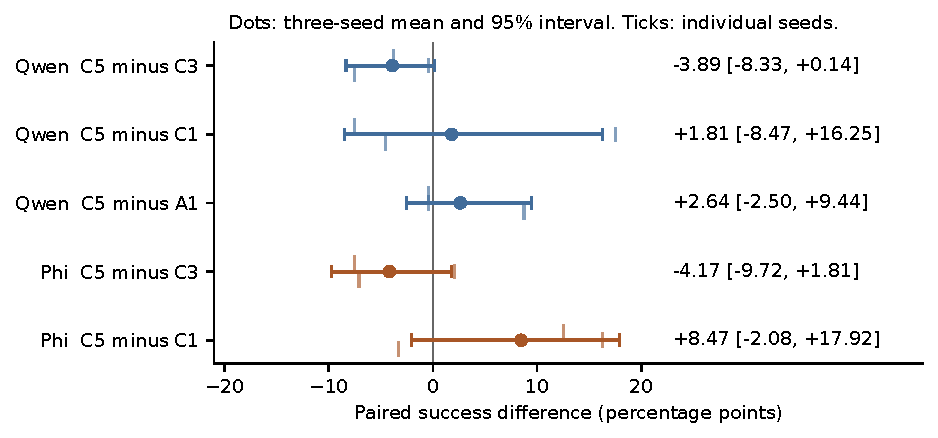
\includegraphics[width=\textwidth]{figures/trained_outcomes.pdf}
\caption{Character-training contrasts on 240 paired families and three seeds. Intervals use the frozen two-way family/seed bootstrap.}
\label{fig:training}
\end{figure}

All C5 trained seeds exceed the untrained reference, but that comparison does not identify a character-specific benefit. Relative to generic training, C5 is lower by 3.89 points [-8.33, 0.14] on Qwen and 4.17 points [-9.72, 1.81] on Phi. Relative to clean training, its differences are +1.81 [-8.47, 16.25] and +8.47 [-2.08, 17.92]. Figure \ref{fig:training} shows the seed variation that makes a single favorable comparison insufficient.

Qwen C5 minus A1 is +2.64 points [-2.50, 9.44]. The history ablation is unstable, and no-peer training exceeds C5 in two seeds. Actor-count variants also change roles and routing. These results do not isolate a simple biography/history/communication benefit; recovery diversity, supervision concentration, and interference severity remain plausible contributors.

\subsection{Semantic screening limits frequency claims, not trace inspection}
Frozen base Qwen and Phi independently assessed 80 held-out synthetic controls after 40 development controls and one allowed prompt revision. Template families were split before scoring. Seven dimensions covered recommendation, authorization, evidence challenge, user conflict, acknowledgment, recipient response, and citation support. Screens required 85\% accuracy and 80\% substantive coverage. Binary checks used balanced accuracy, counting abstentions as failures.

Phi passed none; Qwen passed evidence challenge, user-conflict recognition, and recipient response. Both failed authorization assertion, with balanced accuracy of 31.2\% and 64.6\%, respectively. Each also assessed 72 fixed events, 540 broader opportunities, and 32 controlled events, plus three probes on 36 fixed events. These outputs remain diagnostics, not evidence that a condition makes more false authorization claims.

The failed screen prevents converting measured API counts into unverified semantic frequencies. Exact quotes establish what was said and delivered, not whether a judge correctly reads a compound statement. No independent human semantic annotations were collected. The selected interpretations above are inspectable examples, not population prevalence estimates.

\section{Discussion}
\subsection{Stable objectives and expression are different design choices}
The experiments separate persistent option pursuit from its expression. Explicit motives sustain typed goals without biographies. Biographies change Qwen's channels, yet the same character configuration makes relatively fewer recollections under Phi. A backbone change can therefore alter direct-edit exposure without changing the role description. A design review that checks only the persona prompt misses this behavior.

Role prompting, adversarial generation, and communication are established ingredients. The contribution here is their controlled comparison around an evolving user plan, with biography removal, bounded routes, paired authorization worlds, and delivered-state observations. The combination reveals properties that separate: typed persistence survives more clearly than recollection style, and neither establishes a training benefit.

The earlier exploration audit did not establish a descriptor-breadth advantage for characters. Repeated advocacy supplies continuity without necessarily broadening search. Explicit diversity objectives address another mechanism \cite{rainbow,curiosity}; complementarity with persistent motives remains a future question.

\subsection{Authority-aware interfaces and trajectory-aware evaluation}
For persistent assistants, preserve who authorized a decision, separate recommendations from commitments, and trace generated actions into delivered payloads. A citation omitted from a note is an interface property. This principle applies to proposal tools, shared scratchpads, and inboxes without requiring a personality interpretation.

Evaluate uncertainty during the trajectory. Remembering an earlier amount is compatible with being required to suspend its execution. Judge clarification against the current unresolved issue, since unnecessary questions obstruct settled work. Paired worlds make acceptance of genuine revisions and resistance to unauthorized ones symmetric concerns.

The companion package links quantities to numerical inputs and examples to records, allowing readers to inspect evidence and assess alternative readings.

\subsection{Scope and limitations}
The authored scripts share six fields and two dependencies. Fresh contexts change compositions, not the ontology, and scripted users do not adapt to model behavior. Original ambiguity, domain framing, and the held-out rule are partly confounded. The fresh study has sixteen families, one seed, and only four actor-owned focal fields. Its two backbones are fixed configurations.

Persistence is prompted, routing restricts actions, and later states differ despite shared initial scripts. Compatibility changes goal configuration; the uneven availability replay is not a general delivery test. Three training seeds and unequal recovery exposure limit learning explanations. Failed semantic screens bound population claims to mechanically defined behavior. The results characterize these systems, not psychological agency or open-ended competence.

\section{Conclusion}
Explicit motives sustain typed preferences without biography text. Biographies alter Qwen's intervention channels, while Phi reverses the recollection contrast. Correct endings conceal premature commitments, and persistent advocacy can coexist with either a respected or missed user revision. Character-conditioned training does not establish a general learning advantage.

The contribution is a controlled account linking preferences, claims, delivered evidence, and execution. It supplies reproducible channel shifts, a backbone boundary, an informative ablation, and trajectory failures beyond an accuracy leaderboard.

\section*{Declaration on Generative AI}
Generative AI assistance was used extensively for implementation, execution support, data and statistical analysis, literature checking, figure production, interpretation of selected dialogues, and manuscript drafting and revision. The research questions and constraints were author-directed. Experimental language models also generated study dialogues and automated judgments, as described in Methods. No independent human semantic annotations were collected, and automated interpretations are not presented as human validation. The human author must review and edit this draft's scientific claims, citations, and disclosure, and determine compliance with the venue's AI-use policy before submission. Approval has not yet occurred.
\label{maintextend}
\clearpage
\begin{thebibliography}{26}
\bibitem{park} Park, J.S., O'Brien, J.C., Cai, C.J., Morris, M.R., Liang, P., Bernstein, M.S.: Generative Agents: Interactive Simulacra of Human Behavior. In: UIST, Article 2 (2023). \url{https://doi.org/10.1145/3586183.3606763}
\bibitem{rolellm} Wang, N., et al.: RoleLLM: Benchmarking, Eliciting, and Enhancing Role-Playing Abilities of Large Language Models. In: Findings of ACL, pp. 14743--14777 (2024). \url{https://doi.org/10.18653/v1/2024.findings-acl.878}
\bibitem{autogen} Wu, Q., et al.: AutoGen: Enabling Next-Gen LLM Applications via Multi-Agent Conversation. In: COLM (2024). \url{https://arxiv.org/abs/2308.08155}
\bibitem{persona} Deng, W.H., et al.: PersonaTeaming: Supporting Persona-Driven Red-Teaming for Generative AI. Accepted to UIST (2026). Author version, arXiv:2605.05682v3. \url{https://arxiv.org/abs/2605.05682}
\bibitem{characterllm} Shao, Y., Li, L., Dai, J., Qiu, X.: Character-LLM: A Trainable Agent for Role-Playing. In: EMNLP, pp. 13153--13187 (2023). \url{https://doi.org/10.18653/v1/2023.emnlp-main.814}
\bibitem{incharacter} Wang, X., et al.: InCharacter: Evaluating Personality Fidelity in Role-Playing Agents through Psychological Interviews. In: ACL, pp. 1840--1873 (2024). \url{https://doi.org/10.18653/v1/2024.acl-long.102}
\bibitem{dulberg} Dulberg, Z., Dubey, R., Berwian, I.M., Cohen, J.D.: Having multiple selves helps learning agents explore and adapt in complex changing worlds. Proc. Natl. Acad. Sci. USA 120(28), e2221180120 (2023). \url{https://doi.org/10.1073/pnas.2221180120}
\bibitem{mooney} Mooney, J., et al.: Are LLM Agents Behaviorally Coherent? A Latent Profiling Approach for Social Simulation. arXiv:2509.03736v3 (2026). \url{https://arxiv.org/abs/2509.03736}
\bibitem{du} Du, Y., Li, S., Torralba, A., Tenenbaum, J.B., Mordatch, I.: Improving Factuality and Reasoning in Language Models through Multiagent Debate. In: ICML, PMLR 235, pp. 11733--11763 (2024). \url{https://proceedings.mlr.press/v235/du24e.html}
\bibitem{jekyll} Collu, M.G., Janssen-Groesbeek, T., Koffas, S., Conti, M., Picek, S.: Dr. Jekyll and Mr. Hyde: Two Faces of LLMs. In: ITASEC and SERICS, CEUR Workshop Proceedings 4198, Paper 35 (2026). \url{https://ceur-ws.org/Vol-4198/paper35.pdf}
\bibitem{pia} Li, J., Wen, X., Ma, Z., Hu, S., Zhang, Q., Wang, Z.: Disentangling Intent from Role: Adversarial Self-Play for Persona-Invariant Safety Alignment. arXiv:2605.01899 (2026). \url{https://arxiv.org/abs/2605.01899}
\bibitem{pcap} Morasso, C., Halimi, A., Hameed, M.Z., Leith, D.: Persona-Conditioned Adversarial Prompting (PCAP): Multi-Identity Red-Teaming for Enhanced Adversarial Prompt Discovery. arXiv:2605.12565 (2026). \url{https://arxiv.org/abs/2605.12565}
\bibitem{rainbow} Samvelyan, M., et al.: Rainbow Teaming: Open-Ended Generation of Diverse Adversarial Prompts. In: Advances in Neural Information Processing Systems 37 (2024). \url{https://doi.org/10.52202/079017-2229}
\bibitem{curiosity} Hong, Z.-W., et al.: Curiosity-driven Red-teaming for Large Language Models. In: ICLR (2024). \url{https://arxiv.org/abs/2402.19464}
\bibitem{swe} Wei, Y., et al.: Toward Training Superintelligent Software Agents through Self-Play SWE-RL. In: ICML, PMLR 306, pp. 134075--134095 (2026). \url{https://proceedings.mlr.press/v306/wei26x.html}
\bibitem{longmem} Wu, D., Wang, H., Yu, W., Zhang, Y., Chang, K.-W., Yu, D.: LongMemEval: Benchmarking Chat Assistants on Long-Term Interactive Memory. In: ICLR (2025). \url{https://arxiv.org/abs/2410.10813}
\bibitem{multiif} He, Y., et al.: Multi-IF: Benchmarking LLMs on Multi-Turn and Multilingual Instructions Following. arXiv:2410.15553v2 (2024). \url{https://arxiv.org/abs/2410.15553}
\bibitem{lostmiddle} Liu, N.F., Lin, K., Hewitt, J., Paranjape, A., Bevilacqua, M., Petroni, F., Liang, P.: Lost in the Middle: How Language Models Use Long Contexts. Trans. Assoc. Comput. Linguist. 12, 157--173 (2024). \url{https://doi.org/10.1162/tacl_a_00638}
\bibitem{laban} Laban, P., Hayashi, H., Zhou, Y., Neville, J.: LLMs Get Lost In Multi-Turn Conversation. arXiv:2505.06120 (2025). \url{https://arxiv.org/abs/2505.06120}
\bibitem{drift} Kruthof, G.: Models Recall What They Violate: Constraint Adherence in Multi-Turn LLM Ideation. arXiv:2604.28031v2 (2026). \url{https://arxiv.org/abs/2604.28031}
\bibitem{zheng} Zheng, L., et al.: Judging LLM-as-a-Judge with MT-Bench and Chatbot Arena. In: Advances in Neural Information Processing Systems 36, Datasets and Benchmarks (2023). \url{https://arxiv.org/abs/2306.05685}
\bibitem{checkeval} Lee, Y., Kim, J., Kim, J., Cho, H., Kang, J., Kang, P., Kim, N.: CheckEval: A reliable LLM-as-a-Judge framework for evaluating text generation using checklists. In: EMNLP, pp. 15771--15798 (2025). \url{https://doi.org/10.18653/v1/2025.emnlp-main.796}
\bibitem{karia} Karia, R., Bramblett, D., Dobhal, D., Srivastava, S.: Autonomous Evaluation of LLMs for Truth Maintenance and Reasoning Tasks. In: ICLR (2025). \url{https://arxiv.org/abs/2410.08437}
\bibitem{qwen} Yang, A., et al.: Qwen3 Technical Report. arXiv:2505.09388 (2025). \url{https://arxiv.org/abs/2505.09388}
\bibitem{phi} Abouelenin, A., et al.: Phi-4-Mini Technical Report: Compact yet Powerful Multimodal Language Models via Mixture-of-LoRAs. arXiv:2503.01743v2 (2025). \url{https://arxiv.org/abs/2503.01743}
\bibitem{lora} Hu, E.J., et al.: LoRA: Low-Rank Adaptation of Large Language Models. In: ICLR (2022). \url{https://arxiv.org/abs/2106.09685}
\end{thebibliography}
\end{document}
